\documentclass[conference]{IEEEtran}
\IEEEoverridecommandlockouts
% The preceding line is only needed to identify funding in the first footnote. If that is unneeded, please comment it out.
\usepackage{cite}
\usepackage{amsmath,amssymb,amsfonts}
\usepackage{algorithmic}
\usepackage{graphicx}
\usepackage{textcomp}
\usepackage{xcolor}
\def\BibTeX{{\rm B\kern-.05em{\sc i\kern-.025em b}\kern-.08em
    T\kern-.1667em\lower.7ex\hbox{E}\kern-.125emX}}
\begin{document}

\title{Documentation of Lab work for group 8\\
}

\makeatletter
\newcommand{\linebreakand}{%
  \end{@IEEEauthorhalign}
  \hfill\mbox{}\par
  \mbox{}\hfill\begin{@IEEEauthorhalign}
}
\makeatother

\author{\IEEEauthorblockN{Wiktor Kochanek}
\IEEEauthorblockA{\textit{Electronic Engineering Student} \\
\textit{Hochschule Hamm-Lippstadt}\\
Lippstadt, Germany \\
wiktor.kochanek@stud.hshl.de}
\and
\IEEEauthorblockN{Vytaras Juraska}
\IEEEauthorblockA{\textit{Electronic Engineering Student} \\
\textit{Hochschule Hamm-Lippstadt}\\
Lippstadt, Germany \\
vytaras.juraska@gmail.com}
\linebreakand
\IEEEauthorblockN{Given Name Surname}
\IEEEauthorblockA{\textit{dept. name of organization (of Aff.)} \\
\textit{Hochschule Hamm-Lippstadt}\\
City, Country \\
email address or ORCID}
\and
\IEEEauthorblockN{Alexander Wilms}
\IEEEauthorblockA{\textit{Electronic Engineering Student} \\
\textit{Hochschule Hamm-Lippstadt}\\
Lippstadt, Germany \\
alexander.wilms@stud.hshl.de}}

\maketitle

\begin{abstract}
This document is a record of our group activity and progress in a lab assignment - build an autonomous car.
\end{abstract}

\section{Introduction}
Motivated by a class assignement our group was tasked with creating a self-driving vehicle.
We achieved this by using line tracking sensors and ultrasonic sensors controlled by an Arduino and also implemented a video stream using Raspberry Pi and its external Raspberry Pi Camera V2.

\section{Analyzing the specifications}

Our assignment came with clearly defined specifications:
\begin{itemize}
\item Line tracking system
\item Ultrasonic sensor integration
\item Camera streaming system
\end{itemize}
We split these objectives into two sections: car focused - line tracking and ultrasonic sensors systems - and camera focused - the streaming.
We then split the tasks inside our group so that each member can focus on a specific objective to bring the best possible results.


\section{Car focused specifications}
\subsection{Line tracking system}
The car was supposed to be able to follow a line around a track using two line tracking sensors. The specific implementation of such function was left to our own choice.
We decided to make a system that would allow the car to drive when it doesnt detect a line and react when it does detect a line.

\subsection{Ultrasonic sensors system}
The car was supposed to integrate a system using three ultrasonic sensors - what said system would influence was left to us to decide.
we settled on an obstacle avoiding system that would co-operate with the line tracking system - if there was an obstacle on the track the car
would attempt to drive around the obstacle and drive back onto the track.

\section{Camera focused specification}
The car was supposed to integrate a camera and a system, that would allow it to stream the video from the camera to an external device. The methods of implementation were left to us to decide.
For this task we used a Raspberry Pi with a camera module as a client sending frames and a Mac computer as a server receiving frames and opening them in a format of a picture one by one.

\section{Hardware Architecture}
\subsection{RaspberryPi}
For this project in the case of the video streaming component, we used the versatile single-board-computer named RaspberryP Model 3. The RaspberryPi series in general is worldwide used and shows the practicality in many different use cases globally. One of the main points is that it is promoted to teach the basics of computer sciences in schools, universities and in developing countires. Most of our group members have heard or even worked with a RaspberryPi before, which is a plus. However it is simple to understand and the initial training is fast. As it is a linux based system the commands and functions are simliar to other linux systems. The flexibility of this mirocomputer makes it perfect for rapid protyping in genreral but also perfect for our creation of a self-driving vehicle because we are able to adapt and change parts in the future. The RaspberryPi is also used in the domain of informatics, robotics and electronic engineering but is also interesting for hobbyists who want build projects for themselves. The small price point of under 40 Euros makes it suitable for a lot of people getting in the field. This is a motivation for us to use it and see what the hardware is capable of with our knowledge and work. This way we can publish our code to GitHub and make it public, so other people and students can build their version of a self driving vehicle with a camera stream. It is commonly kown that many people are using and have used the RaspberryPi for surveilance systems, video recordings and streaming projects. We want to give it a try and see if the project is usable for car streaming scenario with a short delay.
\newline
As stated before the car streaming is realized on a RaspberryPi 3. The hardware parts, input/output possiblities and specs are quite remarbale for its size and price. The project definitely benefits from these parts but it has to be noted that the RPi Model 3 might be overpowered for our simple stream of 320x240 pixels. Nevertheless the power of the hardware could be usefull for future adaptations. 
\begin{figure}[h!]
	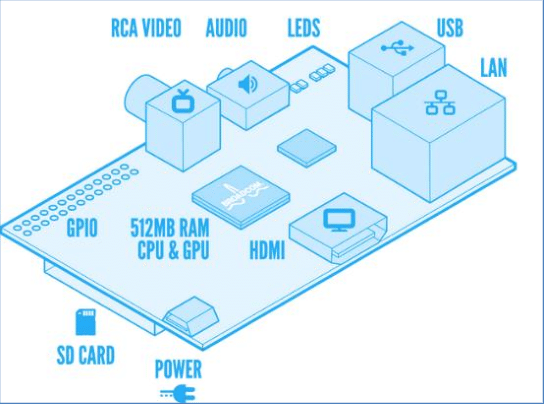
\includegraphics[width=\linewidth]{RPiArchitecture.png}
	\caption{Rough Architecture of RPi}
	\label{fig:RPi}
\end{figure}
The Raspberry Pi features a 64-bit Broadcast System on a chip (SoC) with an integrated ARM-compatible central processing unit (CPU) and on chip graphic processing unit (GPU). The Processor Speed is 1.4 GHz and an on-board memory of 512 MB SDRAM. It also features a Bluetooth and Wifi functionality used for the TCP stream. The Rpi has a 5V/2.5A DC power input which is connected to a power bank. The Extended 40-pin GPIO header was not used but could be useful in further modifactions. The streaming aspect was realized with the CSI camera port and the Camera Module v2. The Full Size HDMI Port is used to connect to a PC monitor to change parameters or the code. It could also be used to stream videos/images  directly on a smaller display directlly mounted on the car. 
\subsection{Camera module}
The focus of a autonomous car/selfdriving vehicle is to process information and react fast. To get to this point, the engineering aspect requires optimezed hardware and software components. We used the powerful Microcomputer RaspberryPi and the official RaspberryPi camera module v2. 
\begin{figure}[h!]
	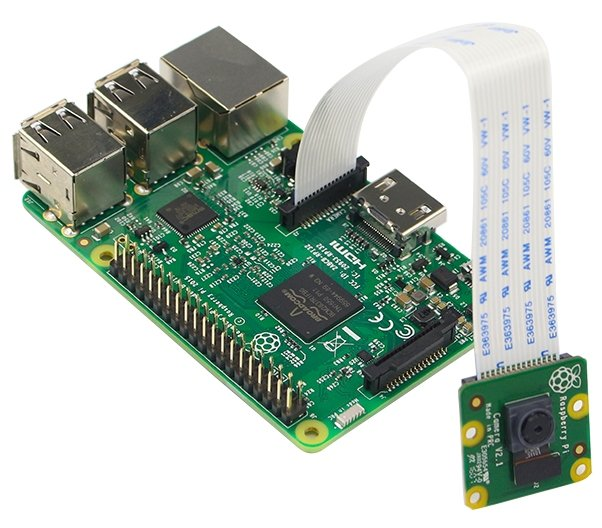
\includegraphics[width=\linewidth]{CameraModule.png}
	\caption{A Connected Camera Module to RPi}
	\label{fig:CMRPi}
\end{figure}
These components are connected via ribbon cable to the special CSI camera port for optimized compatability. The camera in it self is small and well constructed. It has a Sony IMX219 8-megapixel sensor. The Module v2 can be used to used to take still images as well as high-defintion video. It supports  1080p 30fps, 720p 60fps and VGA 90 fps video modes. The camera is easy to use but has many functions for more complicated tasks. There are lots of examples and tutorials on github and other sites, where people show of the capability of the camera by using it for time-lapse, slow-motion and other video effects. There is also the possibility to use libraries and open source projects. 
\newline
The car requires a fast and reliable stream for the user and system. This is why we decided use lightweight protocols like TCP, Berkley Sockets and a small but suffiecient image size of 320x240 pixels. This way we reached a delay of less than 50ms. But before the camera system can be used, setting up the device has to be done. The RaspberryPi has many suitable operating systems, but we chose the official distribution "Raspbian" because it is the most supported and the most efficient operating system for RPi. After downloading the "Raspian Stretch with Desktop" operating system in a format of a .zip file, the image needs to be written on the SD card. We decided to use the program called "Balena Etcher" which, after some complicatinons, in the end worked as intended. After the image is written, and a functional and bootable operating system has been successfuly launched, it is required to enable the camera software, in order to use the camera module. This can be done by the following steps: in the "Prefernces menu" there is a "RaspberryPi Configuration Window", in the "Interface Tab" is the option to "enable Camera". After these steps are completed and reboot is done, the RPi is ready to recognise, use and grant access to the Camera Module.

\section{System Design}
\subsection{Car focused System Design}
The car will operate within 4 states for line tracking system and a pseudostate for the ultrasonic sensors sytem. Different enviromental inputs will influence the behaviour of the car.
\begin{figure}[h!]
	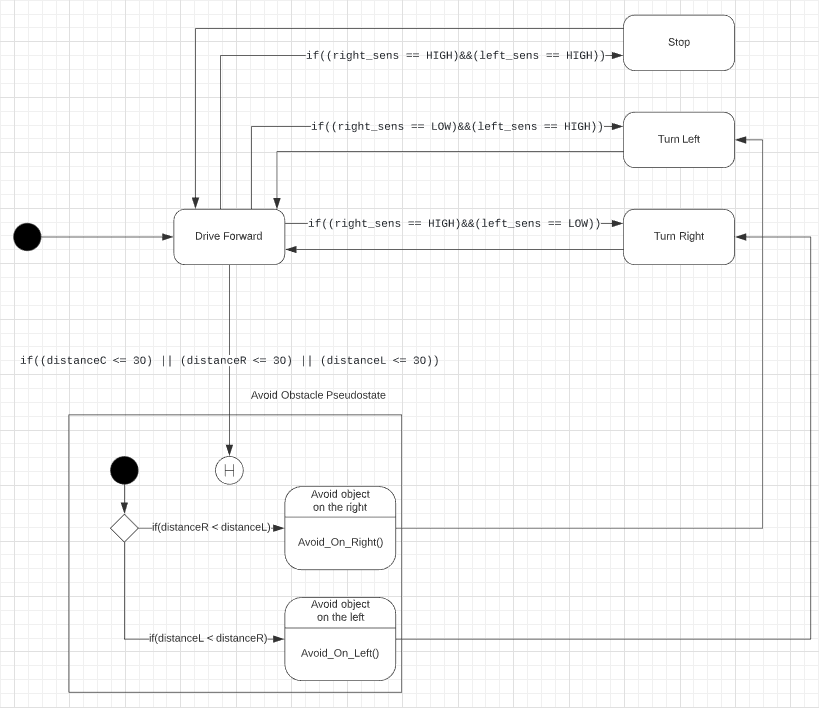
\includegraphics[width=\linewidth]{UMLStateDiagram.png}
	\caption{UML State Diagram}
	\label{fig:UMLSD1}
\end{figure}
The car will always begin in the line tracking state attempting to go forward. When one of the line tracking sensors detects that it has gone onto the line it will steer the car to get the sensor back off the line - Turn Right and Turn Left states. If it happens that both sensors are on the line at the same time the car will stop. Should the cars ultrasonic sensors detect an obstacle it will enter into the Avoiding Obstacles Pseudostate. It will then decide if the obstacle is closer to its right or left side and will attempt to avoid the obstacle on the other side. When it succesfully returns to the track the line tracking sensors will exit the car from the pseudostate and will reutrn line tracking functionality.

\subsection{Video steam focused System Design}
Since specifications did not define what methods of implementation had to be used, we really wanted to implement OpenCV into our video streaming system, hence our system design was focused more on the implementation methods with
OpenCV. After some reaserch of how does the main concept of video streaming look like, we decided to settle on our finalised base concept of our video streaming system design.
\begin{figure}[h!]
	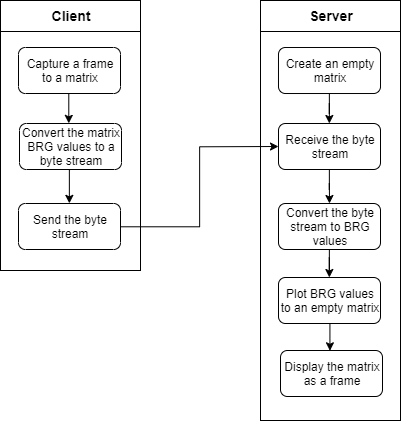
\includegraphics[width=\linewidth]{StreamConceptActivityDiagram.png}
	\caption{Video Streaming System Design}
	\label{fig:VSSD1}
\end{figure}
The idea for the client was to portray frames as matrixes, in which every single pixel would be a component with 3 channels in the sequence of Blue, Red and Green. We portray each channel in a byte value with a limited amount of bits dedicated to each channel component. So our client has to store each frame in a matrix, convert every single matrix component channel into a byte stream and send the byte stream over to the server. From the server side the process is a bit lengthier, first it has to create an empty matrix, as a template. After the server receives the byte stream from the client, it has to convert the byte stream back to the channels, which would resemble each component in the matrix. After plotting each component sequentially back to the matrix template, we would receive a whole frame, which we finally can open up as an image.

\section{Implementation of the system}
\subsection{Line tracking system}
The line tracking system was the first thing tackled in the car functionality. The first implementation was a simple use of "if" and "if else" functions - depending on which line tracking sensor was tirggered, speeds of motors would change to make the car drive forward, turn the correct way or stop completely. Later implementation made use of interrupts, which changed the motor speed in the interrupt service routine.
\begin{figure}[h!]
	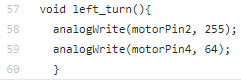
\includegraphics[width=\linewidth]{examplecode1.png}
	\caption{used interrupt service routine$^{1}$}
	\label{fig:EXC1}
\end{figure}
\footnote{lines of code in Fig. 2 do not represent actual content in the final source code}
While the interrupt solution was a great way to make the source code easy to understand and the car ran very smoothly, it was scrapped during integration with ultrasonic sensor code as there were compatiblity problems. As such we settled on a "if" and "if else" functions solution.
\subsection{Obstacle avoidance system}
Implementation of the ultrasonic sensors was not specifically defined in the project requriements. Our design used them in a way to detect and obstacle in the way and attempt to drive around it. First the car had to know that there was an obstacle in front of it. This was achieved simply using an "if" function - if any of the three sensors detect an obstacle within 30cm of the car they will trigger the if condition and enter the car in the pseudostate of "avoid obstacle".
\begin{figure}[h!]
	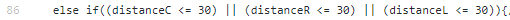
\includegraphics[width=\linewidth]{examplecode2.png}
	\caption{if condition detecting the obstacle}
	\label{fig:EXC2}
\end{figure}
After the car enter this pseudostate we have to choose which way is best to avoid the obstacle on - meaning that if theres a wall on our right, we want to turn to the left to clear it and vice versa. This is simply done by comparing the distance values on the right and left ultrasonic sensors - distanceR and distanceL respecitvelly. In this case we don't care about the centre distance as it doesnt influence our choice of side to avoid on. After the choice is made the car enters a loop that lets it go around an obstacle - in this example we will be avoiding an obstacle on the right (distanceL $<$ distanceR).
\begin{figure}[h!]
	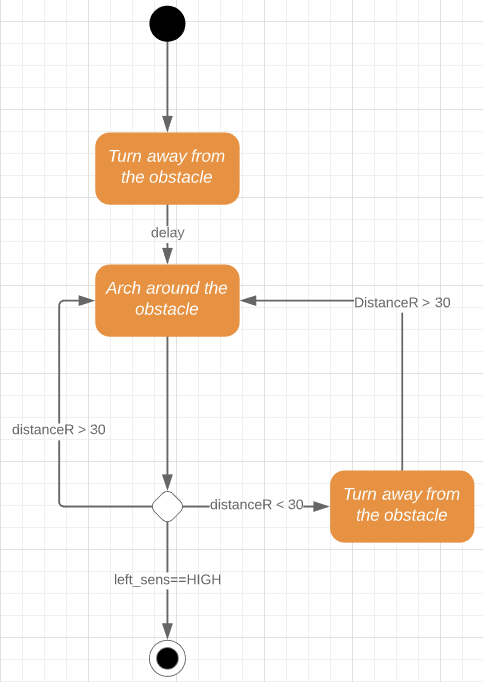
\includegraphics[width=\linewidth]{AvoidActivityDiagram.png}
	\caption{Activity diagram of the avoiding algorithm}
	\label{fig:AAD}
\end{figure}
After starting the avoiding algorithm the car will slowly arch around its obstacle. it is possible that the obstacle is longer than the arch diameter, so the car is able to detect obstacles in this mode and turn away again if needed.
This algorithm was designed to allow the car to leave its line in order to avoid the obstacle and detect when it is supposed to once again follow said line. In order to do that we had to have the car ignore one of the line tracking sensors for the duration of avoiding algorithm - in this case the right line tracking sensor - and then respect the sensor again when it gets back on the line. This was simply done by running the algorithm in a subfunction and including a simple if condition in the loop. The car arching around the obstacle is implemented using a while loop that relies on a variable set after the car decides on which side is the obstacle. The only way to stop that while loop is the active line tracking sensor - in this case the left one - to cross onto the line. The sensor triggering ends the while loop and the avoidance algorithm returning the car to its line tracking functionality.
\subsection{Video stream system}
Since we wanted to implement OpenCV into our video streaming system, we decided to make it in C++ programing language. As a method of communication, with no doubts we chose TCP Internet Protocol and it's implementation in C++ programming - Berkeley Sockets, which we, at the time, recently learned from the lectures and were really motivated to implement it into our video streaming.
\newline
The first problem we encountered, was what to use, to compile OpenCV and Berkeleys Sockets in C++. After trying out many popular IDE's (Integrated Development Enviroment) on a Windows based device, we decided to start the development purely on our Raspberry Pi, which was running on Raspbian, Debian-based opperating system. Since we finally started working on Raspbian, all we had to do, was to install OpenCV libraries, dedicated for Raspberry Pi, and compiling was not an issue anymore. After we could finally compile our code properly, we started learning how Berkeley Sockets worked and how to implement a client and a server successfuly, since we had implementation in our lectures, the process was not complicated, but fully understanding it and changing properties in a way, that the communication would function as intended was challenging. Once we understood the basics of Berkeley Sockets, we started implementing OpenCV to Berkeley Sockets. Since we had a bit of prior experience with OpenCV, we did not have to learn it from the basics, so we instantly went for implementation. After countless trial and error, we finally got it to work:

\subsubsection{Client system}
Before any task was performed, the client has to check if the camera was aviable. That was easily done by implementing OpenCV class, called "VideoCapture"
\begin{figure}[h!]
	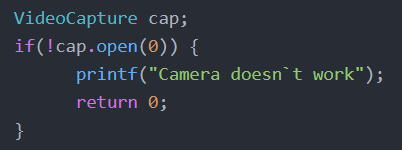
\includegraphics[width=\linewidth]{ClientCodeExample1.png}
	\caption{Camera access check}
	\label{fig:CCE1}
\end{figure}
which has many functions dedicated for camera access. One of the functions is called "open", which if parameters of the funcion "open" are not zero, that means there was no access to the camera or there was an error.
\newline
Going forward the code enters an infinite loop, which would be the whole process of connecting, capturing frames, converting to byte stream, sending byte stream. First we begin from creating a Socket.
\begin{figure}[h!]
	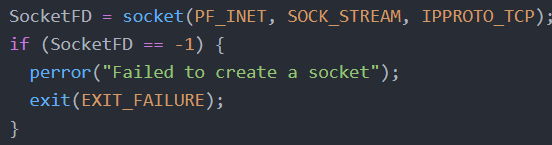
\includegraphics[width=\linewidth]{ClientCodeExample2.png}
	\caption{Socket creation in Client}
	\label{fig:CCE2}
\end{figure}
We define what a socket is and all of its properties are, simply put, referring to the type of protocol, which has to be used, which in our case is TCP. Later on we check, if we were successful in creating a socket.
\newline
Afterwards, using "inet\_pton" function, we have to connect to the server knowing the socket address, port and it's IP (Internet Protocol). Just then we can finally connect our socket using the "connect" function
\begin{figure}[h!]
	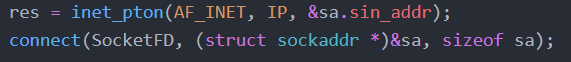
\includegraphics[width=\linewidth]{ClientCodeExample3.png}
	\caption{Connecting to Server and connecting the Socket}
	\label{fig:CCE3}
\end{figure}
\newline
And if we finally have connected to the server, we can start capturing the frame, converting it and sending it to the client.
\begin{figure}[h!]
	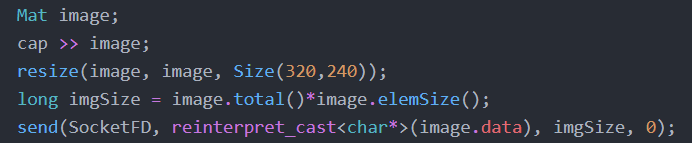
\includegraphics[width=\linewidth]{ClientCodeExample4.png}
	\caption{Capturing the frame, converting and sending to Server}
	\label{fig:CCE4}
\end{figure}
First we create a matrix, which we use to store the frame, when we capture it with already predefined "VideoCapture" class variable. We resize the image to 320 by 240 pixels to improve the speed of sending the byte stream and calculate the final image size, which is later on needed in the "send" function. The final function "send" is a bit more tricky, first we dedicate the already connected socket as a socket for sending, dedicate the message property, which in our case are matrix components converted to a long byte stream, and shortened by "reinterpret\_cast", define the already calculated size of the message, which is the size of the frame, and declare the flag, which we never needed to play around with, so we left it at zero. The tricky part of "send" function is the "reinterpret\_cast", because this type of operator is not safe, it does not check if pointer type and the data, which the pointer is pointing at, are the same or not, which can harm the device, if an error in pointers occur, or the types of variables in the code are mixed up.
\newline
That is where a single cycle of the loop ends and this is the core of the client system.
\subsubsection{Server System}
Majority of functions, which are in the client system, are reused in the server system as well. Firstly (same as in Fig. 7), we create a TCP socket and check, if the creation was successful. Then we try to bind the socket to the socket address and the dedicated port, through which our client will try to connect to the server.
\begin{figure}[h!]
	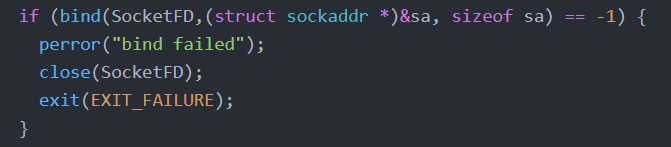
\includegraphics[width=\linewidth]{ServerCodeExample1.png}
	\caption{Binding the socket}
	\label{fig:SCE1}
\end{figure}
 If the binding has failed (for example the port is in use), then we close the socket, we've been trying to open, and terminate the program.
\newline
This is where the infinite loop from the server side starts and its starts of with the function "listen". It's properties, are the socket, which to check for incoming connections, and the maximum incoming connections allowed at a single time period. If "listen" function returns negative one, it means, that some sort of error has been made and the socket has to be closed, and the program has to be terminated for security reasons.
\begin{figure}[h!]
	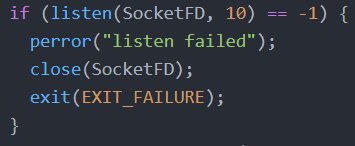
\includegraphics[width=\linewidth]{ServerCodeExample2.png}
	\caption{Listening error check}
	\label{fig:SCE2}
\end{figure}
\newline
Then we create the zero matrix, which is a template with components, which are all empty. We calculate an estimate size of the matrix, to have an exact expected maximum byte stream size, when the server receives it. Before communication both client and the server have to agree on the resolution of the frames, for the frame to be recollected properly from the byte stream. Then we store the recieved data to a variable with a function "recv", which properties are: socket from where it recieves the byte stream, the byte stream itself, the estimate size of the byte stream from the predetermined zero matrix.
\newline
One of the last steps of the loop is the byte stream conversion to the matrix components channel values. The byte stream is stored in a corresponding sequence of channels: Blue, Red, Green. We divide the whole byte stream into segments, where one segment represents one channel value, three of those channels represent a single component of the matrix, which in the end is just a pixel in a frame. So this exact part of the loop divides a byte stream to pixels and sorts them row by row, column by column back into a single frame.
\begin{figure}[h!]
	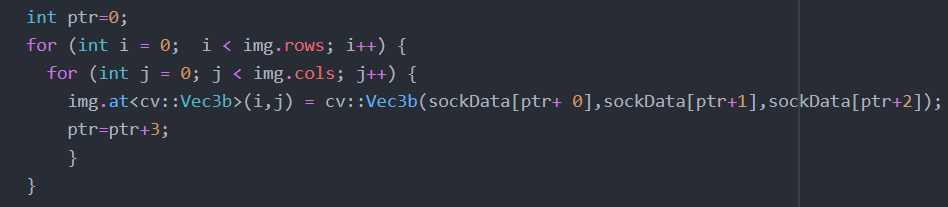
\includegraphics[width=\linewidth]{ServerCodeExample3.png}
	\caption{Byte stream conversion to BRG values}
	\label{fig:SCE3}
\end{figure}
\newline
And the last part of the loop is opening up an already prepared frame with a function "imshow", after a single frame is shown, it has to close after some time, so we have to implement a function "waitKey", which waits for a specified time in miliseconds or completely terminates the program if any key on the keyboard was pressed. If "waitKey" wouldnt be implemented, more and more frames would stack on each other, taking up all the recourses of the device, so this function is necessary.

\section{Evaluation}
\subsection{Camera stream integration}
Even though big portions of the program were outsourced from different implementations and slightly modified to fit our needs and requirements, the results software wise were astonishing. The longer we spent trying to figure out what were missing and what we already have in our code, the more offten we came back to the UML diagrams, the more we started to understand our requirements, what we need to do to achieve them, and how different parts work, when going more into depth of implementation and design. Unfortunately, majority of functions used were parts of different libraries, which we did not thrive to understand, because of time pressure. Never the less, we are still curious and will continue being interested in the topics, which this project covered. It feels like we are just barely starting to understand the possibility of developing and engineering.



\end{document}